\documentclass[conference,final,a4paper,twocolumn,9pt]{IEEEtran}

\usepackage{cmap}
\usepackage[utf8x]{inputenc}
\usepackage[T1]{fontenc}

\usepackage{lmodern}

\usepackage{mathtools}
\usepackage{amssymb}

\usepackage[USenglish]{babel}

\usepackage{array}
\usepackage{amsthm}
\usepackage{amsfonts}
\usepackage{mathtools}
\usepackage{makeidx}
\usepackage[pdftex]{graphicx}
\usepackage{url}
\usepackage{epigraph}
\usepackage{hyperref}
\usepackage{cite} % natbib
\usepackage{flushend}

\ifCLASSINFOpdf
\usepackage[pdftex]{graphicx}
\DeclareGraphicsExtensions{.pdf,.jpeg,.png}
\else
\usepackage[dvips]{graphicx}
\DeclareGraphicsExtensions{.eps}
\fi

\usepackage{amsmath}
\usepackage{algorithmic}
\usepackage{url}

\usepackage{tikz, pgfplots}
\usepackage{tikz-qtree}

\pgfplotsset{compat=1.7}
\usetikzlibrary{patterns}

\begin{document}
\title{RobOptim: an Optimization Framework for Robotics}
%
\author{\IEEEauthorblockN{Thomas~Moulard\IEEEauthorrefmark{1}, %
    Florent~Lamiraux\IEEEauthorrefmark{2}, %
    Karim~Bouyarmane\IEEEauthorrefmark{3}, %
    Eiichi~Yoshida\IEEEauthorrefmark{1}}%
%
\IEEEauthorblockA{\IEEEauthorrefmark{1}%
  CNRS-AIST, JRL (Joint Robotics Laboratory), UMI 3218/CRT,\\%
  Intelligent Systems Research Institute,\\%
  AIST Central 2, Umezono 1-1-1,\\%
  Tsukuba, Ibaraki 305-8568 Japan\\%
  E-mail: \texttt{thomas.moulard@gmail.com}}%
\IEEEauthorblockA{\IEEEauthorrefmark{2}%
  LAAS-CNRS, Universit\'e de Toulouse\\%
  7, avenue du Colonel Roche\\%
  31077 Toulouse cedex 4, France}%
\IEEEauthorblockA{\IEEEauthorrefmark{3}%
  ATR Computational Neuroscience Laboratories,\\%
  Department of Brain Robot Interface,\\%
  2-2-2 Hikaridai, Seika-cho, Soraku-gun,\\%
  Kyoto 619-0288, Japan}%
}%
%
\maketitle

\begin{abstract}
\boldmath Numerical optimization is useful for various areas of
robotics. However tackling optimization problems properly requires the
use of non-trivial algorithms which tuning is challenging. RobOptim
aims at providing a unified framework for different categories of
optimization problems while relying on strong C++ typing to ensure
efficient and correct computations. This paper will present this
software, demonstrates its genericity and illustrates current use by two
full scale robotics examples.
\end{abstract}

\begin{IEEEkeywords}
  Numerical Optimization, Software, Humanoid Robotics
\end{IEEEkeywords}

\IEEEpeerreviewmaketitle

\section{Introduction}\label{sec:introduction}


\IEEEPARstart{O}{ver} the past years, numerical optimization proved
itself particulaly suited for various robotics applications such as
posture or trajectory optimization~\cite{miossec06,saab-tro-12}, robot
control~\cite{mansard-icra-12} and more. These applications yield both
linear and non-linear optimizations problems with equalities and
inequalities constraints. Robot control also relies on other types of
optimization such as quadratic programming. As robot control
algorithms run in real-time, it leads to strong constraints on the
implementation efficiency. The design and implementation of a solver
is tedious and error-prone. Avoiding numerical precision issues,
ensuring that the algorithm behaves properly in all cases even with
ill-conditioned problems is challenging, in particular for roboticists
who are not experts in optimization techniques. Among available
optimization toolboxes, the Matlab Optimization Toolbox~\cite{matlab},
the Open Optimization library, OPT++, IPOPT~\cite{ipopt},
SciPy~\cite{scipy} and the GSL (Gnu Scientific Library)~\cite{gsl} all
provides several optimization algorithms. Unfortunately, these
libraries suffer from several drawbacks: some are difficult to use,
some do no support for advanced algorithms such as support for
constrained optimization or have efficiency issues, etc. They also all
lack a unified model expressing optimization problems.


RobOptim solves these limitations by introducing a framework to model
any continuous optimization problem, constrained or not. The design
is focused on providing an easy to use C++ set of safe and efficient
libraries which can be used to prototype robotics applications.
Let us emphasize here that our framework does not implement any numerical
optimization algorithm. Instead, it provides a model for functions, problems
and solvers on the one hand and plug-ins wrapping existing solvers as CFSQP
or IPOPT on the other hand.
The
RobOptim computational model will be first introduced
in~\autoref{sec:roboptim} and different applications will be detailed
in~\autoref{sec:application}. In particular, an extension of RobOptim
for a particular category of problem has been implemented recently,
demonstrating the ability of RobOptim to support a large variety of
problems. The conclusion will detail advantages and limitations of the
current approach and summarize the roadmap for the next developments.


\begin{figure}[ht!]
  \begin{center}
    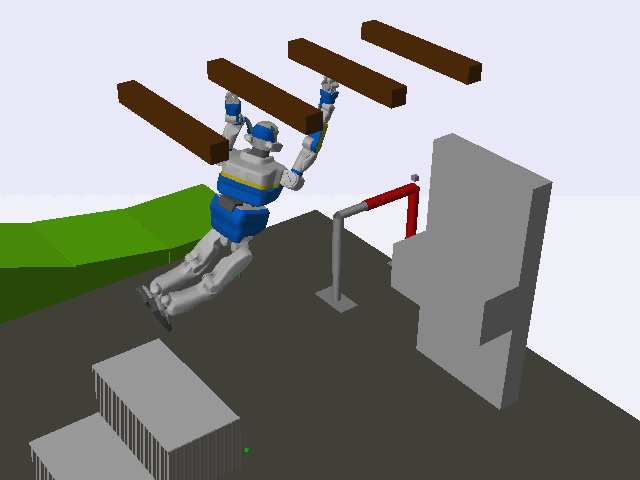
\includegraphics[width=\linewidth]{agent-067.jpg}
    \caption{Posture optimization while considering dynamic
      constraints with RobOptim.\label{fig:stence-optimization}}
  \end{center}
\end{figure}



\section{RobOptim overview}\label{sec:roboptim}


RobOptim is a set of open-source C++ libraries available under the
LGPL license. Code source, documentation and examples are provided by
the project webpage: \mbox{\url{http://www.roboptim.net/}}.


The RobOptim framework is divided into three parts. The core layer
provides a computation model expressive enough to model different
types of optimization problems. The solver layer gathers different
optimization algorithms. The third layer consists in several
application dependent packages bundling reusable mathematical
functions.


\subsection{Mathematical function representation}


Continuous optimization problems can be defined as follow:

\begin{equation}\label{eq:optimization}
  \min_{\mathbf{x} \in \mathbb{R}^n} f(\mathbf{x}) \text{ under the constraint } \mathbf{x} \in \mathbf{X}
\end{equation}

where $f : \mathbb{R}^n \mapsto \mathbb{R}$ is the cost function and
$\mathbf{X} \subset \mathbb{R}^n$ is the space of the admissible
solutions. This space is usually defined by a set of inequality and
equality constraints:

\begin{equation}
  \mathbf{X} \triangleq \left\{
  \begin{array}{l l}
    c_i (x) = 0    & \quad i \in \xi \\
    c_j (x) \leq 0 & \quad j \in \nu \\
  \end{array} \right.
\end{equation}

$c_i$, $c_j$ are respectively the set of equality and inequality
constraints. $i$ and $j$ are the indices identifying the constraints.

The mathematical functions $f$ and $c_k$ ($k \in \xi \cup \nu$) must
provide a way to evaluate their result at any point they are
defined. Their associated gradient and hessian can also be
provided. Finally, each of these function may be catorized as
belonging to a set of functions matching a particular structure which
may help the resolution. One example is linear functions. The goal of
the RobOptim core layer is to express these features through the C++
typing rules.


Depending on the solving algorithm, it may be necessary to obtain the
jacobian and in some cases even the functions hessian. Hence,
functions providing maximum information about themselves will be
compatible with a larger proportion of solvers.

\begin{figure}[ht!]
  \begin{center}
    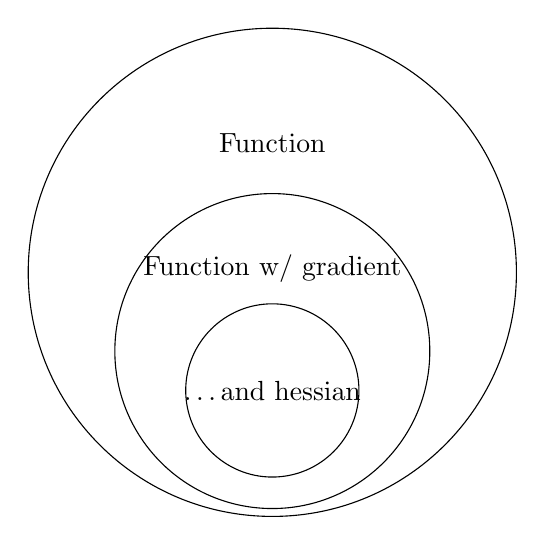
\begin{tikzpicture}
      \draw (0,-1.5) circle (1.1) node {\ldots and hessian} ;
      \draw (0,-1) circle (2) node [above=.75cm] {Function w/ gradient} ;
      \draw (0,0) circle (3.1) node [above=1.4cm] {Function} ;
    \end{tikzpicture}
  \end{center}
  \caption{Sets representing the different kind of functions that
    RobOptim can model out-of-the-box.}\label{fig:functions}
\end{figure}

In RobOptim, each mathematical function is represented by a different
C++ class. All of these types then inherit the abstract kind of
mathematical functions they represent. The following kind of
mathematical functions are bundled with RobOptim core: function that
can evaluate itself (\texttt{Function} type), function that can
evaluate itself and its gradient (\texttt{DifferentiableFunction}),
function that can evaluate itself, its gradient and its hessian
(\texttt{TwiceDifferentiableFunction}), etc.  Let 'A <: B' be the
relationship ``type B is a subtype (subclass) of A'' or ``B inherits
from A''. Then a partial order can be defined where: Function <:
DifferentiableFunction <: TwiceDifferentiableFunction. It can also be
understood through sets as illustrated by~\autoref{fig:functions}.


\subsection{Optimization problem definition and problem resolution}


Once function cost and all constraints functions have been
implemented, an optimization problem has to be built. RobOptim core
provides a meta-class \texttt{Problem} parametrized by two parameters
$F$ and $C_L$. $F$ the cost function type and $C_L$ is the list of the
constraints types. A non-linear problem with constraints then has the
following type:


\texttt{Problem<DerivableFunction, vector<LinearFunction, DerivableFunction > >}


The constraints can be either linear or non-linear. With this
constraints type definition, the constraints will be divided into two
categories which will help the solver perform efficiently.

Additionally, bounds can be set on the optimization variables and a
starting point for the optimization process may be specified. When the
constraints are added to the problem, each one of them is associated
with a validity interval. If this interval is reduced to a point, the
constraint is an equality constraint. At both compile time and
run-time, RobOptim checks that only valid problem are built. For
instance if one add a linear constraint then RobOptim checks at
compile time that the constraint is a subtype of the
$\texttt{LinearFunction}$ type.


Once the problem is defined, a solver that will solve the problem needs
to be instantiated. Each solver is parametrized by the same types as
optimization problems. Therefore the solver $S<P_1,C_{L1}>$ can
solve the problem $P<P_2,C_{L2}>$ if the following relation is true:


\begin{equation}
  P_1 <: P_2 \wedge \forall i, C_{L1}(i) <: C_{L2}(i)
\end{equation}


Basically, the problem can be solved if all types provide enough or
more information than necessary. For instance if gradient are
required, the function may also provide hessian computation but if
gradient is lacking the compile time assertions will fail and prevent
the user from building an invalid optimization problem.

By separating problem expression from solver, dynamic changes of the
solving algorithm are possible. Each solver is bundled as a plug-in
which is loaded at run-time. The interest is to let the user freely change
the problem complexity during the design process. Other
frameworks would require a different API depending on the kind of
optimization at hand, where through RobOptim changes are minimal. One
may choose to use a more powerful than required solver at first and
then refine the choice or implement later a new plug-in providing
the best algorithm for one particular application. These features are
provided through meta-programming techniques and come with a near zero
cost\footnote{RobOptim core does not realize copy so the additional
  runtime cost is only due to calls to virtual functions.} at runtime
and are unique to RobOptim.

\subsection{Cost and constraint toolbox}


Unlike others frameworks where computations are tightly linked to one
problem and one solver, RobOptim abstraction layer allows user to
implement toolboxes of reusable functions. This part of RobOptim is
dedicated to robotics. The ``trajectory'' layer of RobOptim is
currently providing trajectores defined as B-Splines and associated
mathematical functions to realize minimal time optimization for
instance.


\subsection{Toward easy and safe problem design}


RobOptim is heavily relying on templated meta-programming, a C++
language feature allowing notably to defined parametrized types and
execute algorithms at compile time~\cite{iso14882}. By defining
problems and solvers through parametrized types, the compiler is able
to check that the functions that are used to instantiate the
optimization problem are compatible with the type of problem under
construction. Thus, only solvers supporting this kind of problem can be
used. Through meta-programming, these safety checks are evaluated at
compile-time and thus do not impact final performances. Regarding ease
of use, having a unified representation of all models which matches
closely the underlying theory simplifies the understanding of the
implementation process.  To finish, RobOptim relies on modern tools
such as Boost and Eigen to support natural ways of implementing
algebra computation. Additional tools such as gradient checks through
finite differentiation is also provided to help ensuring functions
correctness.


\section{Applications and case study}\label{sec:application}


RobOptim has been used to solve several different types of robotics
problems. The two scenarii that will be detailed here are footsteps
optimization and posture optimization for a humanoid robot. Another
important point is the extensibility of the framework. To demonstrate
RobOptim capacities to adapt to new types of problems an example of
such extension will be given. These experiments aim at generating
motion for the humanoid robot HRP-2~\cite{hrp2}.


\subsection{Step planning for humanoid robots}


Generating a walking motion in an environment cluttered with obstacles
is challenging. One commonly used approach are Rapidly exploring
Random Trees
applied to the robot bounding box or to the robot itself sliding on the ground~\cite{dalibard2011small}.
These probabilistic algorithm will try to create a path
between the starting point and the goal point by sampling
configurations randomly and have the ability to find solutions for
highly dimensioned problems on a reasonable time. However, the
probabilistic nature of these algorithms leads to paths which seems
unnatural. One solution to improve these paths is numerical
optimization. In this application, RobOptim has been used to optimize
a biped robot walking trajectory determined beforehand by a motion
planning algorithm.

Let $\gamma$ be the initial robot waist trajectory defined as a
B-Spline from $t_{min}$ to $t_{max}$. A free time trajectory $\Gamma$
is defined from $T_{min}$ to \linebreak $T_{max} = T_{min} + \lambda
(t_{max} - t_{min})$ as
\begin{equation}
  \Gamma_{\lambda} (T) = \gamma (t_{min} + \frac{1}{\lambda} (T -
  T_{min}))
\end{equation}

\begin{table}[ht!]
  \begin{center}
    \begin{tabular}{|c|l l l| l |l l l|}
      \hline
      Time
      & \multicolumn{3}{|c|}{control point 1}
      & \ldots
      & \multicolumn{3}{|c|}{control point $n$}\\
      \hline
      $\lambda$
      & $x_0$ & $y_0$ & $\theta_0$
      & \ldots
      & $x_n$ & $y_n$ & $\theta_n$\\
      \hline
    \end{tabular}
  \end{center}
  \caption{Optimization variables for walking motion problem\label{fig:optim-param}}
\end{table}


The use of a free time trajectory allows the solver to both optimize
trajectory shape and speed by respectively changing the control points
and the scale $\lambda$. Optimization variables are illustrated
by~\autoref{fig:optim-param}. The free time trajectory derived from
the trajectory $\gamma$ is used as the state of the solver.


\begin{table}[ht!]
  \begin{center}
    \begin{tabular}{|c|c|}
      \hline Cost function & $f(\mathbf{x}) = \lambda$\\ Speed
      constraint & $\forall T, \text{foot},\quad
      (\frac{v_{\text{foot}}^{x}}{v_{\text{max}}^{x}})^2 +
      (\frac{v_{\text{foot}}^{y}}{v_{\text{max}}^{y}})^2 - 1 \leq
      0$\\ Distance constraint & $\forall T,\quad\text{distance} (\text{obstacle},
      \Gamma (T)) > 0$\\ \hline
    \end{tabular}
    \caption{Walking optimization problem formulation\label{fig:pb-walking}}
  \end{center}
\end{table}


The problem cost function is defined as $\lambda$. It corresponds to
minimizing the time by accelerating the trajectory as much as
possible. To preserve a feasible final trajectory while encouraging
forward motion, a speed constraint is added which take separately into
account the front speed $v^x$ and the lateral speed $v^y$ of each foot
of the robot. Another constraint is preventing the robot to
collide with obstacles. The problem definition is detailed
in~\autoref{fig:pb-walking}.


\begin{figure}[ht!]
  \begin{center}
    %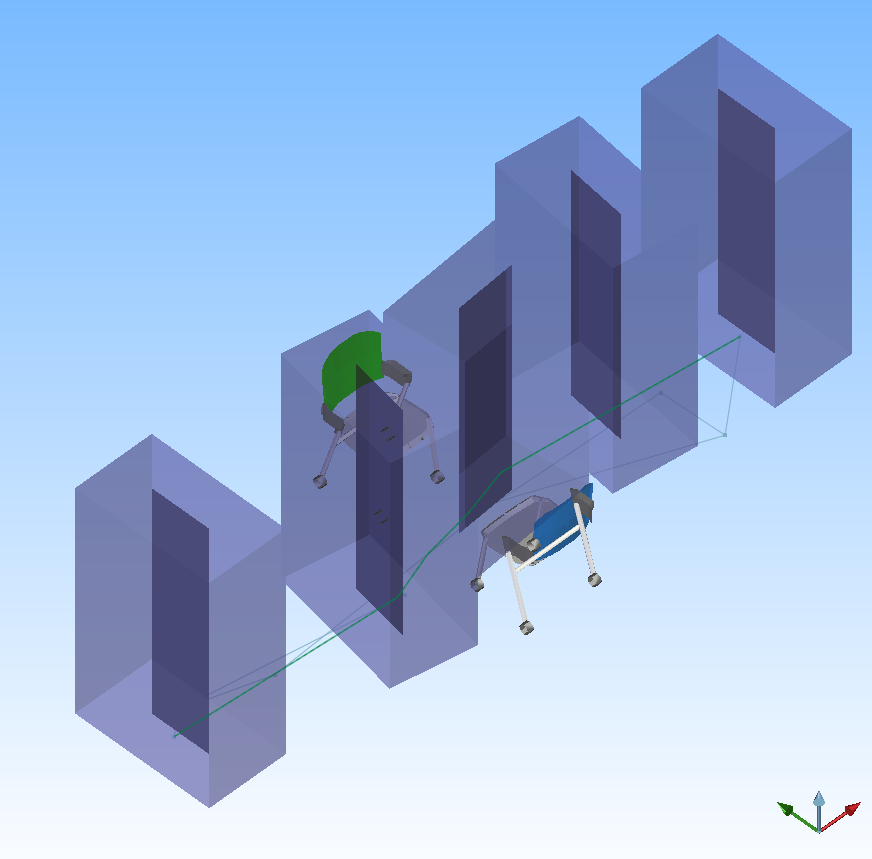
\includegraphics[width=\linewidth]{two-chairs.png}
    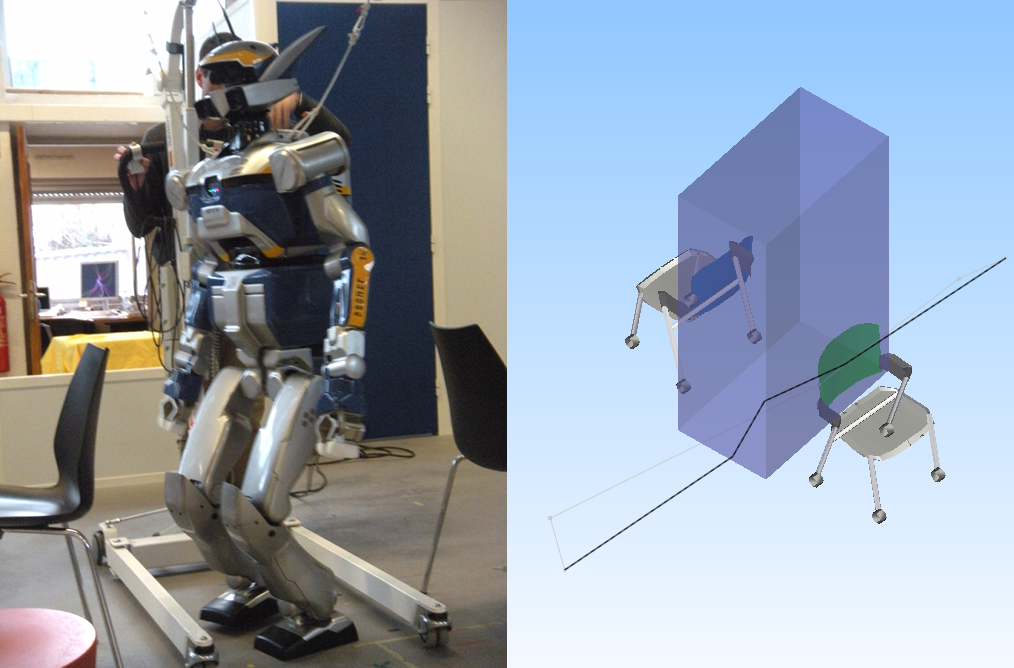
\includegraphics[width=\linewidth]{hrp2-two-chairs.png}
    \caption{Walking trajectory optimization\label{fig:result-walking}}
  \end{center}
\end{figure}


This non-linear problem has been successfully solved by RobOptim while
relying on the proprietary solver CFSQP~\cite{cfsqp} internally and
result is shown on~\autoref{fig:result-walking}.


\subsection{Posture optimization for humanoid robots}


Another problem is posture optimization, which consists in choosing
the best configuration such that a system will accomplish the
objectives it has been assigned. In this example, the goal is to find
a configuration as close as possible to a goal posture while taking
into account various constraints. In this case, robots and environment
objects are considered as elements of the optimization
problem. Constraints include: robot and objects static equilibrium,
Newton's third law, Coulomb friction model, fixed grasp model for
bilateral contact forces, joints limits and torques limits. This
problem is described extensively
in~\cite{Bouyarmane2011a,Bouyarmane2010} and demonstrated the ability
of RobOptim to solve complex large scale non-linear problems.


\subsection{Extending the framework: least square optimization}


Initially, non-linear optimization problems with constraints have been
solved with RobOptim. By providing a generic computational framework,
it is possible to extend RobOptim to support other types of problems
such as least square optimization. A least square optimization problem is an
unconstrained problem the cost function of which is defined by

\begin{equation}
  f(\mathbf{x}) = \sum_{i=1}^m f_i (\mathbf{x})^2
\end{equation}
where $f_1,\cdots,f_m$ are $m$ non-linear differentiable functions from $\mathbb{R}^n$ to $\mathbb{R}$.

To build functions matching this definition, another function type
called \texttt{SumOfC1Squares} has been derived from the
\texttt{DifferentiableFunction} class. The constructor of this new type takes
as input the function from $\mathbb{R}^n$ to $\mathbb{R}^m$ the coordinates of
which are $f_1,\cdots,f_m$. \texttt{SumOfC1Squares} then redefines evaluation
and gradient of $\sum_{i=1}^m f_i (\mathbf{x})^2$.

The CMinPack solver has then
been wrapped into a RobOptim solver class which takes as input problem
of the type: \texttt{Problem<SumOfC1Squares, vector<> >}.

The introduction of this new type of solver did not require any change
in the RobOptim infrastructure and proved the genericity of the
approach.


\section{Conclusion}\label{sec:conclusion}


A new approach to optimization problem representation has been exposed
in this paper. By expressing numerical optimization problems through
C++ typing, the RobOptim optimization framework provides a unified
computational model. Moreover, advanced C++ template meta-programming
techniques preserve efficiency while giving the capacity to express
high-level mathematical objects such as cost functions and
constraints. These features have been proved useful to solve different
types of robotics problem. Even while being generic, the RobOptim core
layer suffers from limitions. It still lacks support for optimization
in non-scalar spaces such as $\text{SO}(3)$. By importing knowledge
about the structure of the optimization variables, solvers could
realize more efficient computation. For instance, \mbox{3D} rotations
can be represented by homogeneous matrices, quaternions, vectors and
angles, etc. Switching from one representation to another may lead to
better convergence and a decrease in the number of necessary
mathematical operation. One goal would be to both be able to express
information regarding the optimization variables structure and find a
method to help solvers rely on these additional information. To
achieve this level of expressiveness, modern C++ feature is of great
help and no optimization framework is providing yet such features when
it comes to design an optimization problem.


Therefore, RobOptim is a step forward toward making optimization
techniques available for non-expert by providing easy to understand
and generic model, strong C++ object model ensuring safety and
toolboxes bundling robotics oriented functions that may be reused when
one builds its own optimization problem.


\bibliographystyle{IEEEtran}
\bibliography{IEEEabrv.bib,robomec13.bib}

\end{document}
